\documentclass[a4paper,11pt,twocolumn]{article}

\usepackage[UTF8,fontset=fandol]{ctex}
\usepackage{amsmath,amssymb}
\usepackage{graphicx}
\usepackage{booktabs}
\usepackage{geometry}
\usepackage{hyperref}
\usepackage{caption}
\usepackage{array}
\usepackage{float}
\usepackage{xcolor}

\graphicspath{{work2/}{work4/}{work5/}{final_figures/}}
\geometry{a4paper,margin=1.78cm,columnsep=0.82cm}
\setlength{\parindent}{2em}
\setlength{\parskip}{0.22em}
\setlength{\textfloatsep}{9pt plus 1pt minus 2pt}
\setlength{\floatsep}{8pt plus 1pt minus 2pt}
\setlength{\intextsep}{8pt plus 1pt minus 2pt}
\renewcommand{\arraystretch}{1.08}
\captionsetup{font=small,skip=2pt}

\renewcommand{\thesection}{第\arabic{section}章.}
\renewcommand{\thesubsection}{\arabic{section}.\arabic{subsection}}

\title{\vspace{-0.8em}\textbf{人工神经网络课程综合报告}\\
\large 从迁移学习到古文数学语言模型的神经网络实验整理}
\author{方俊睿\\学号：3230104069}
\date{}

\begin{document}
\maketitle
\vspace{-1.0em}

\begin{abstract}
本文从长学期课程报告中选取三份完成度较高、实验记录较完整的报告进行压缩整理：Food101 图像分类中的从头训练与微调对比、《九章算术》字符级语言模型与文本嵌入、《孙子算经》领域大模型微调与偏好后训练。三份报告表面上覆盖视觉分类、传统序列模型和大语言模型，核心问题却是一致的：神经网络如何在有限数据和有限算力条件下获得可迁移的表示、可验证的性能提升和可解释的领域知识。综合结果表明，预训练和结构先验能显著提高训练效率；小规模领域语料可以让模型学习格式、术语和单位体系，但严格推理能力仍需更强的数据设计和评价方法支撑。本文按“统一视角、三份报告、课程总结”的结构组织，使三份独立作业被压缩为一篇连续的课程论文。
\end{abstract}

\noindent\textbf{关键词：}迁移学习；语言模型；文本嵌入；Qwen3；DPO；古文数学文本

\section{以一个统一的视角简述三份报告}

本学期的多个实验可以统一理解为一个问题：当任务数据、训练时间和硬件资源都受到限制时，神经网络应当依靠什么获得有效泛化。本文选择的三份报告分别位于这一问题的三个层次。第一份报告研究 Food101 图像分类，直接比较随机初始化训练与 ImageNet 预训练微调，重点是迁移特征能否提升分类精度并降低训练成本。第二份报告面向《九章算术》文本，使用字符级 LSTM 和 Skip-gram 嵌入观察小型模型能否学习古代数学文本中的题答格式、数字单位和语义共现。第三份报告进一步使用 Qwen3 0.6B 与 Unsloth，在《孙子算经》上完成从头训练、SFT 和 DPO，比较小模型从零学习与预训练大模型领域适配之间的差异。

三份报告的共同线索不是模型规模越来越大，而是“表示如何形成”。在视觉任务中，表示主要来自大规模自然图像预训练；在《九章算术》实验中，表示来自字符序列统计与题答监督；在《孙子算经》实验中，表示先由通用大模型提供，再通过 LoRA/QLoRA 和偏好优化向特定领域收缩。若只看最终准确率或生成样例，三类实验似乎难以比较；但若从数据、模型、训练目标、评价指标四个方面观察，就可以看到一致的工程逻辑：先建立可靠基线，再通过可控对照证明改动的收益，最后承认指标无法覆盖的能力边界。

为了让三份报告在同一篇文档中具有连续性，本文采用“任务约束--模型先验--训练目标--评价边界”的横向框架来组织内容。任务约束回答“数据有多少、标签或答案是否可靠”；模型先验回答“模型从哪里获得初始能力”；训练目标回答“优化过程实际奖励了什么行为”；评价边界回答“当前指标不能说明什么”。这个框架能把视觉分类和语言生成放在同一张分析图中，也能避免把不同任务的指标直接进行不恰当比较。

\begin{table}[H]
\centering
\scriptsize
\caption{三份报告的统一比较}
\resizebox{\columnwidth}{!}{
\begin{tabular}{llll}
\toprule
报告 & 任务 & 核心方法 & 主要评价 \\
\midrule
报告一 & Food101 分类 & 迁移微调对照 & Acc、F1、耗时 \\
报告二 & 《九章算术》生成与嵌入 & LSTM、Skip-gram & PPL、关键词、近邻 \\
报告三 & 《孙子算经》大模型 & Qwen3 SFT、DPO & loss、生成对比 \\
\bottomrule
\end{tabular}}
\end{table}

最终选取这三份，是因为它们的数据、脚本、图表和结果分析都较完整，也能形成一条从判别式视觉模型到生成式语言模型、再到现代大模型后训练的清晰主线。相比之下，基础 MLP 报告更偏课程入门与调参验证，GAN 报告可视化完成度较好但定量评价较弱，因此未作为综合报告主体。

更具体地说，报告一提供了最标准的监督学习对照：数据规模较大、指标清晰、四组实验可横向比较。报告二把问题从分类转到序列建模，模型规模不大，但数据处理、损失曲线、生成样例和嵌入近邻都能说明模型实际学到了什么。报告三则接近当前深度学习工程实践，包含从头训练、指令微调和偏好优化三个阶段，能与前两份报告形成技术层次上的递进。三者合在一起，不只是把三个作业拼接起来，而是展示了课程中反复出现的一个判断：模型能力必须放在数据、先验、训练目标和评价指标的关系中理解。

\begin{table}[H]
\centering
\scriptsize
\caption{三份报告被选入综合文档的理由}
\resizebox{\columnwidth}{!}{
\begin{tabular}{lll}
\toprule
报告 & 优点 & 可压缩后的主线价值 \\
\midrule
Food101 & 指标完整、对照明确 & 说明迁移学习的效率收益 \\
《九章算术》 & 有生成、嵌入和曲线 & 说明小模型如何学习领域模式 \\
《孙子算经》 & 覆盖 SFT 与 DPO & 说明大模型后训练的能力和边界 \\
\bottomrule
\end{tabular}}
\end{table}

\begin{table}[H]
\centering
\scriptsize
\caption{本文采用的横向评价框架}
\resizebox{\columnwidth}{!}{
\begin{tabular}{llll}
\toprule
维度 & 报告一 & 报告二 & 报告三 \\
\midrule
任务约束 & 101 类图像分类 & 古文题答生成 & 小语料大模型适配 \\
模型先验 & ImageNet 预训练 & 字符序列结构 & Qwen3 通用能力 \\
训练目标 & 交叉熵分类 & 答案续写与共现 & SFT 与偏好优化 \\
主要风险 & 过拟合与类别混淆 & 记忆题型模板 & 偏好数据过窄 \\
\bottomrule
\end{tabular}}
\end{table}

\section{报告1：Food101 图像分类中的从头训练与微调}

\subsection{任务背景与实验设计}

第一份报告研究视觉分类中的一个典型工程问题：在中等规模数据集上，是从随机初始化开始训练，还是使用预训练模型微调。实验选择 Food101 数据集，包含 101 类食物图像。训练集原始规模为 75750，测试集为 25250；训练集内部按 9:1 划分训练与验证集。输入图像统一调整为 $224\times224$，训练阶段使用随机裁剪和水平翻转，验证与测试阶段使用中心裁剪，并采用 ImageNet 归一化。

模型选择 ResNeXt50\_32x4d 与 DenseNet121。每个模型分别设置 scratch 和 finetune 两种训练方式，共四组对照。统一优化器为带 momentum 的 SGD，损失函数为交叉熵，评价指标为 Top-1 Accuracy 与 Macro-F1。微调采用两阶段策略：先冻结 backbone 训练分类头，再解冻全网并对 backbone 使用更小学习率。这样既能利用预训练特征，又能避免一开始大步长更新破坏通用表示。

这个实验的关键不是单独追求最高精度，而是让四组实验尽量可比。若同时改变模型、优化器、数据增强和训练轮次，最终结果很难归因；因此报告固定了输入尺寸、归一化方式、损失函数、优化器类别和主要评价指标，只改变“模型结构”和“是否使用预训练”。这种控制变量的设计使后续结论更接近实验事实，而不是经验判断。

\begin{table}[H]
\centering
\scriptsize
\caption{Food101 统一训练配置}
\begin{tabular}{ll}
\toprule
项目 & 配置 \\
\midrule
输入尺寸 & $224\times224$ \\
训练增强 & RandomResizedCrop + HorizontalFlip \\
验证/测试 & Resize + CenterCrop \\
损失函数 & CrossEntropyLoss \\
优化器 & SGD, momentum=0.9 \\
权重衰减 & $1\times10^{-4}$ \\
评价指标 & Top-1 Accuracy, Macro-F1 \\
训练设备 & CUDA, 2 GPU, AMP \\
\bottomrule
\end{tabular}
\end{table}

\subsection{主要结果}

\begin{table}[H]
\centering
\scriptsize
\caption{Food101 四组实验结果}
\resizebox{\columnwidth}{!}{
\begin{tabular}{lcccc}
\toprule
实验 & best val acc & test acc & test F1 & train(h) \\
\midrule
ResNeXt-scratch & 0.7283 & 0.7857 & 0.7852 & 3.31 \\
ResNeXt-finetune & 0.7533 & 0.7978 & 0.7957 & 2.63 \\
DenseNet-scratch & 0.7373 & 0.7937 & 0.7933 & 6.74 \\
DenseNet-finetune & 0.7757 & 0.8240 & 0.8230 & 5.48 \\
\bottomrule
\end{tabular}}
\end{table}

\begin{figure}[H]
\centering
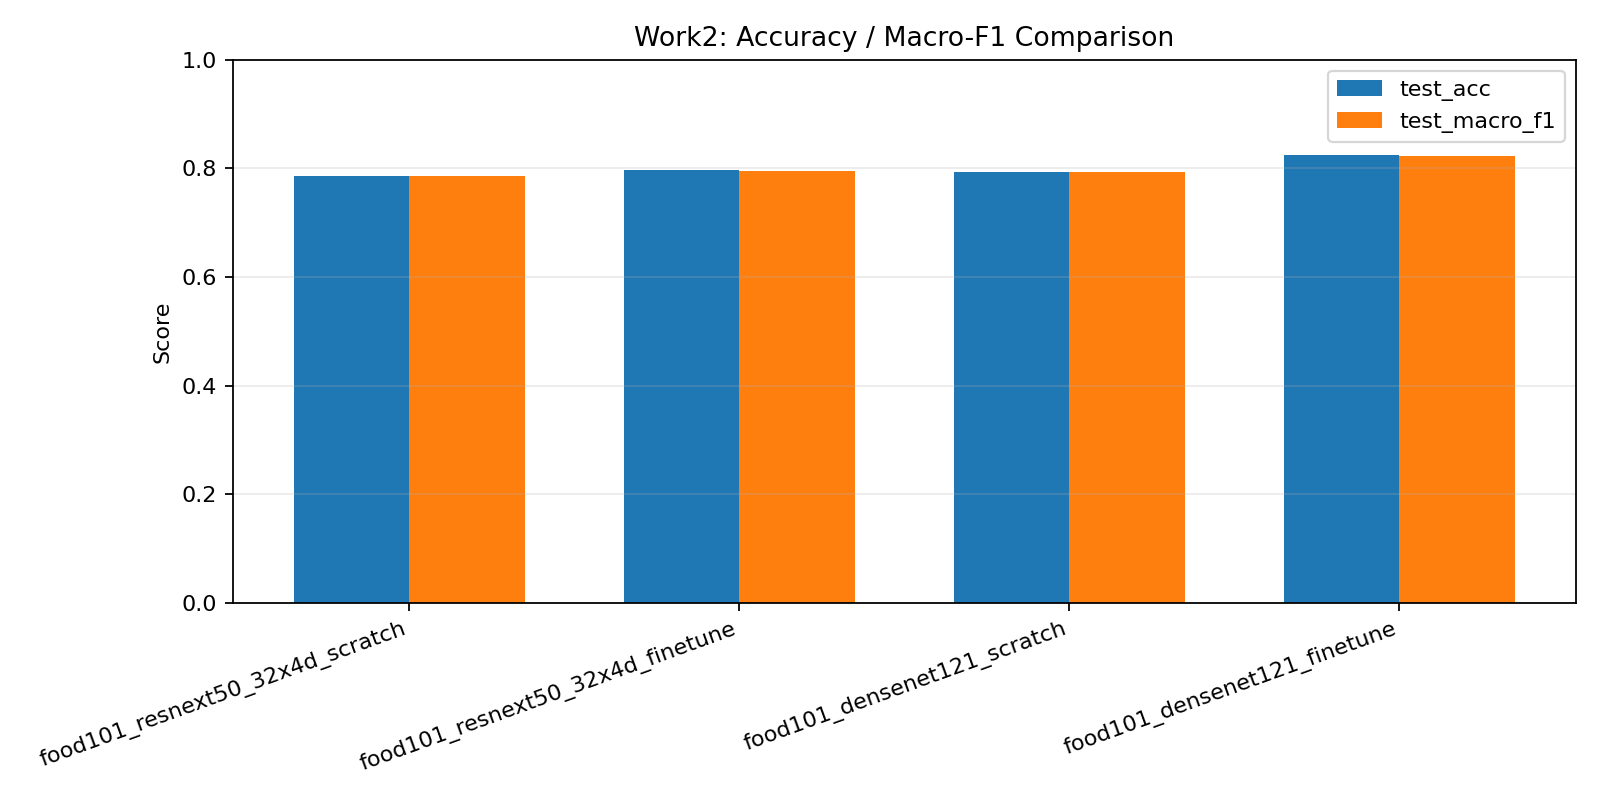
\includegraphics[width=\columnwidth]{work2_compare_acc_f1.png}
\caption{Food101 中四组实验的 Accuracy 与 Macro-F1}
\end{figure}

结果显示，微调在两种模型上都稳定优于从头训练。ResNeXt 的测试准确率从 0.7857 提升到 0.7978，DenseNet 的测试准确率从 0.7937 提升到 0.8240。Macro-F1 的变化与 Accuracy 基本一致，说明提升并非只来自少数大类。训练成本方面，ResNeXt 微调耗时由 3.31 小时降至 2.63 小时，DenseNet 由 6.74 小时降至 5.48 小时，说明预训练不仅提升最终性能，也改善收敛效率。

从收敛过程看，微调更早进入高精度区间。ResNeXt 和 DenseNet 的微调实验达到“最佳验证准确率的 95\%”分别在第 23、21 轮，而 scratch 需要第 32、33 轮。微调两阶段中，冻结分类头阶段完成新类别适配，解冻后验证准确率明显跃迁，说明 backbone 的通用特征经过低学习率调整后能够进一步贴合 Food101 的类别边界。

\begin{table}[H]
\centering
\scriptsize
\caption{收敛速度与泛化差距对比}
\resizebox{\columnwidth}{!}{
\begin{tabular}{lccc}
\toprule
实验 & 达到 95\%最佳值 epoch & 最佳 val epoch & 末轮 train-val gap \\
\midrule
ResNeXt-scratch & 32 & 59 & +0.1400 \\
ResNeXt-finetune & 23 & 47 & -0.0488 \\
DenseNet-scratch & 33 & 56 & +0.0942 \\
DenseNet-finetune & 21 & 50 & -0.0406 \\
\bottomrule
\end{tabular}}
\end{table}

表中 train-val gap 的方向也值得注意。scratch 实验末轮训练准确率明显高于验证准确率，说明模型已经开始更强地贴合训练集；而 finetune 的末轮 gap 为负，一方面可能来自较强数据增强使训练集在线样本更难，另一方面也说明预训练初始化下验证性能更稳定。这个现象提示：在中等数据规模上，预训练并不只是“更快开始”，还可能通过更好的初始表示降低过拟合风险。

\subsection{分析与结论}

本实验最清楚的结论是：在 Food101 这样的中等规模视觉任务上，预训练微调是更优先的训练方案。DenseNet121-finetune 是四组中的最佳组合，test acc 达到 0.8240，Macro-F1 达到 0.8230。DenseNet 的密集连接可能更有利于细粒度食物图像中的纹理和局部形状复用，因此在本实验中表现优于 ResNeXt。

同时，本实验也保留了必要的谨慎。所有结果只基于单次随机种子，尚未报告均值与方差；scratch 的学习率和正则化搜索不够充分，可能低估了从头训练上限；错误分析也还停留在整体指标，缺少混淆矩阵和类别级诊断。因此，该报告的意义主要在于通过公平对照说明迁移学习的稳定收益，而不是证明某一网络结构在 Food101 上达到最优。

从课程学习角度看，报告一给出的经验是：视觉任务中的“模型好坏”必须拆成若干层次。第一层是最终测试集表现，第二层是收敛速度，第三层是训练成本，第四层是过拟合与泛化差距。只有四层同时观察，才能判断一个训练策略是否真的更值得采用。在本实验中，微调在四个层次上都占优，因此结论比较坚实。

如果把该报告扩展为更完整的研究，还可以增加两类实验。一类是统计可靠性实验，即使用多个随机种子重复训练，报告均值和标准差；另一类是错误结构实验，即输出混淆矩阵和类别级准确率，分析哪些食物类别最容易混淆。前者解决“结果是否稳定”的问题，后者解决“模型错在哪里”的问题。课程作业中受限于训练时间，这两点只作为改进方向保留。

\section{报告2：《九章算术》语言模型与文本嵌入}

\subsection{任务背景与数据处理}

第二份报告转向文本建模，目标是在课程规模内观察神经网络能否从《九章算术》中学习古文数学题的表达模式。原始文本包含大量“题面--答曰--答案”结构，适合构造条件生成任务。预处理首先处理编码差异，依次尝试 UTF-8、GB2312、GB18030 和 GBK；随后统一异体写法、清理空白，并按编号块抽取题答对。最终得到 452 条题答对，按随机种子划分为 385 条训练样本和 67 条验证样本。

本报告包含两个互补模型。第一个是字符级 LSTM 语言模型：输入为题面和“答曰：”，目标是在答案位置计算交叉熵并生成后续文本。选择字符级建模，是因为古文数学文本包含繁体字、数字、单位和固定句式，分词会引入额外不稳定性。第二个是 Skip-gram Negative Sampling 嵌入模型，用窗口共现关系学习字符向量，并通过近邻检索观察数学术语之间的语义关系。

这里的数据处理本身就是实验的重要部分。古文数学文本不是现代结构化数据，题目编号、标点、异体字、换行和编码都会影响样本抽取。报告中没有直接把整篇文本喂给模型，而是先识别“题面”和“答案”的边界，再把“题面 + 答曰：”作为条件上下文，把答案部分作为主要监督目标。这样做虽然增加了预处理复杂度，但能让训练目标更贴近“根据题目生成答案”这一任务，而不是简单地做无条件续写。

\subsection{模型配置与评价指标}

LSTM 使用 256 维 embedding、2 层 512 隐藏维度，训练 300 轮，优化器为 AdamW。评价时记录验证交叉熵、困惑度，并在验证题目上生成答案。为了避免只依赖主观阅读，报告设计了答案关键词命中率：从标准答案中提取数字和单位，例如“一、二、十、百、分、步、畝、頃、尺、升、斗”等，若生成文本覆盖至少一半关键词则记为命中。该指标不能等同于数学正确率，但能衡量模型是否学到了答案格式和单位体系。

Skip-gram 模型使用 128 维字符嵌入、窗口大小 4、负样本数 8，训练 40 轮。它不直接生成答案，而是从共现结构角度回答另一个问题：模型是否能把“粟、米、尺、寸、田、步”等字符放入合理的数学语境中。

LSTM 的训练目标可写为
\[
\mathcal{L}_{\mathrm{LM}}=-\sum_t \log p(x_{t+1}|x_{\leq t}),
\]
其中题面部分主要提供条件，答案部分贡献更直接的监督信号。Skip-gram 负采样则近似优化中心字符与上下文字符的相似度：
\[
\mathcal{L}_{\mathrm{SGNS}}=-\log\sigma(v_w^\top u_c)
-\sum_{i=1}^{K}\log\sigma(-v_w^\top u_{n_i}).
\]
两个目标的差异决定了它们的解释方式：LSTM 更适合看生成结果和困惑度，Skip-gram 更适合看近邻结构。

\begin{table}[H]
\centering
\small
\caption{《九章算术》模型结果}
\resizebox{\columnwidth}{!}{
\begin{tabular}{lcc}
\toprule
模块 & 指标 & 数值 \\
\midrule
LSTM & 最优验证 epoch & 41 \\
LSTM & 最优验证 loss / PPL & 1.0663 / 2.9045 \\
LSTM & 答案关键词命中率 & 0.9000 \\
Skip-gram & token 数量 & 59239 \\
Skip-gram & 训练样本对 & 473892 \\
Skip-gram & 最终 loss & 2.3327 \\
\bottomrule
\end{tabular}}
\end{table}

\begin{figure}[H]
\centering
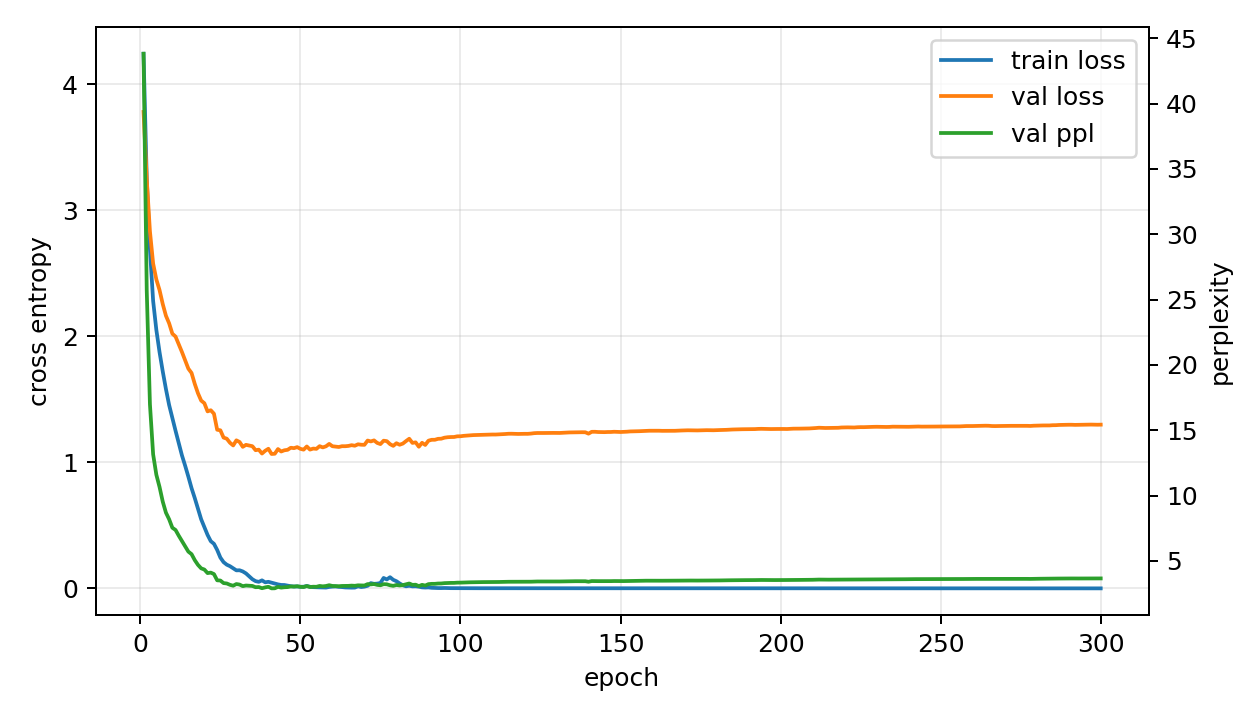
\includegraphics[width=\columnwidth]{work4_lstm_curves.png}
\caption{《九章算术》字符级 LSTM 训练曲线}
\end{figure}

\begin{table}[H]
\centering
\scriptsize
\caption{LSTM 生成样例}
\resizebox{\columnwidth}{!}{
\begin{tabular}{lll}
\toprule
题型摘要 & 标准答案 & 生成答案 \\
\midrule
田廣十五步，從十六步 & 一畝 & 一畝 \\
九十一分之四十九 & 十三分之七 & 十三分之七 \\
股四尺，弦五尺，求句 & 三尺 & 三尺 \\
井徑五尺，不知其深 & 五丈七尺五寸 & 五丈七尺五寸 \\
共買豕，人出一百盈一百 & 一十人 & 一十人 \\
\bottomrule
\end{tabular}}
\end{table}

\subsection{生成与嵌入结果}

训练曲线显示，验证损失在第 41 轮达到最低，此后训练损失继续下降而验证损失上升，说明模型开始记忆训练集。最终保存的是验证损失最低的模型。生成样例中，一些结构固定、题型高频的问题可以得到完全一致的答案，例如“田廣十五步，從十六步”生成“一畝”，“九十一分之四十九”约分生成“十三分之七”，“股四尺，弦五尺，求句”生成“三尺”。这些结果说明模型确实学习到了一部分题型模板、古文数字表达和单位格式。

嵌入模型的近邻也提供了侧面证据。“粟”的近邻集中在粮食换算相关语境，“尺”的近邻包括“寸、丈、深、竿、绳”等长度相关字符，“答”的近邻接近“问、何、曰”等问答结构符号。这表明即使是轻量级字符嵌入，也能从《九章算术》的局部共现中学到一定领域结构。

\begin{table}[H]
\centering
\scriptsize
\caption{Skip-gram 近邻结果示意}
\begin{tabular}{ll}
\toprule
查询字符 & 近邻解释 \\
\midrule
粟 & 粮食、米、饭食换算相关语境 \\
米 & 饭、稻、米制品和粮食单位相关 \\
尺 & 寸、丈、深、竿、绳等长度语境 \\
田 & 頃、步等面积和田亩计算语境 \\
答 & 问、何、曰等题答结构语境 \\
\bottomrule
\end{tabular}
\end{table}

不过，该报告也明确区分了文本模式学习与算术推理。LSTM 能复现常见题型，不代表它真正执行了通用计算；当题目涉及低频换算或价格关系时，模型容易迁移其他题型的答案。关键词命中率较高，也只能说明单位和数字模式被捕捉，不能保证答案数值严格正确。后续若要验证推理能力，应构造“题型不变、数字替换”的合成测试集，以排除记忆训练样例的影响。

因此，报告二的价值主要在于展示“小模型如何被正确使用”。它没有把 LSTM 描述成能解决古代数学题的通用推理器，而是把模型能力限定在题答格式、单位表达、常见题型模板和字符共现关系上。这种限定反而提高了报告可信度：模型能做什么、不能做什么，都有对应证据。

这一部分也提醒我，传统模型仍然适合教学和分析。相比大模型，LSTM 的训练曲线、验证损失拐点和过拟合现象更直观；Skip-gram 的近邻表虽然简单，却能直接观察字符共现关系。在课程学习阶段，这种可解释性很重要，因为它帮助我理解神经网络并不是“自动理解文本”，而是在特定目标函数下压缩和复用统计规律。

\section{报告3：《孙子算经》领域大模型训练}

\subsection{任务背景与框架选择}

第三份报告进一步进入现代大模型微调。课程要求在 nanoGPT、MiniMind、Unsloth 三个框架中任选一个，完成从头训练、至少 Qwen3 0.6B 规模模型的微调，以及后训练实验。报告最终选择 Unsloth，是因为它对 Qwen3、4-bit 加载、LoRA/QLoRA 和 DPO 的支持更直接，适合在有限显存下完成完整流程。

\begin{table}[H]
\centering
\scriptsize
\caption{框架选择的比较}
\resizebox{\columnwidth}{!}{
\begin{tabular}{lll}
\toprule
框架 & 优势 & 本实验取舍 \\
\midrule
nanoGPT & 简洁透明，适合理解 GPT 训练 & 缺少现代微调封装 \\
MiniMind & 中文小模型流程较完整 & 适合系统复现但配置较重 \\
Unsloth & 支持 Qwen3、QLoRA、DPO & 最贴合作业要求 \\
\bottomrule
\end{tabular}}
\end{table}

数据集使用《孙子算经》文本。该文本包含古文数学题、度量衡单位和大量“答曰”格式，非常适合构造指令微调数据。数据准备阶段生成三类文件：完整规范化文本用于从头训练，messages 格式 JSONL 用于 SFT，prompt/chosen/rejected 格式 JSONL 用于 DPO。其中 rejected 通过扰动数字或单位自动构造，表达“原文答案优于错误数字或错误单位答案”的偏好。

数据格式的拆分也反映了三个训练阶段的目标差异。从头训练使用连续文本，目的是让随机初始化模型学习字符分布；SFT 使用 user/assistant 格式，目的是让预训练模型学会“题目到答案”的交互形式；DPO 使用 chosen/rejected，目的是进一步表达输出偏好，使模型倾向于短答案、正确单位和原文风格。三者使用同一原始文本，但监督信号逐步增强。

\begin{table}[H]
\centering
\scriptsize
\caption{《孙子算经》数据格式}
\resizebox{\columnwidth}{!}{
\begin{tabular}{lll}
\toprule
数据文件 & 用途 & 监督信息 \\
\midrule
pretrain.txt & 从头语言建模 & 连续文本统计 \\
sft.jsonl & 指令微调 & 题目到标准答案 \\
dpo.jsonl & 偏好后训练 & chosen 优于 rejected \\
\bottomrule
\end{tabular}}
\end{table}

\subsection{从头训练、SFT 与 DPO}

从头训练部分使用小型 decoder-only Transformer，字符级建模，6 层、8 个注意力头、隐藏维度 384。它的作用不是得到最强模型，而是作为完整训练流程和小语料局限性的基线。结果显示训练 loss 可以快速下降，但验证 loss 和 PPL 很高，说明模型在 65 条题答对规模下容易记忆训练集，泛化不足。

SFT 阶段使用 Qwen3 0.6B 4-bit 基础模型，通过 QLoRA 只训练低秩 adapter。LoRA rank 为 16，alpha 为 32，目标模块覆盖注意力投影和 MLP 投影层。微调输入采用 chat template，将题目作为 user 消息，将原文“答曰”后的内容作为 assistant 回复。DPO 阶段从 SFT adapter 初始化，使用 chosen/rejected 偏好对继续训练。报告中记录到初始 400 steps 的 DPO 容易在小偏好集上造成重复生成，最终改为 50 steps、$1\times10^{-5}$ 学习率，使输出保持稳定。

LoRA/QLoRA 的作用可以理解为在大模型中插入小规模可训练参数。基础模型主体保持冻结，低秩矩阵负责学习领域差异。这样做牺牲了一部分完全自由更新的能力，但显著降低显存占用和训练成本，也降低了小数据集上破坏通用能力的风险。对本实验这样只有几十条题答对的任务而言，参数高效微调比全参数微调更合理。

\begin{table}[H]
\centering
\small
\caption{《孙子算经》大模型实验结果}
\resizebox{\columnwidth}{!}{
\begin{tabular}{lcc}
\toprule
阶段 & 指标 & 数值 \\
\midrule
数据准备 & 题答对数量 & 65 \\
从头训练 & 最终验证 loss / PPL & 6.9084 / 1000.64 \\
Qwen3 SFT & train loss & 0.1377 \\
Qwen3 DPO & step / lr & 50 / $1\times10^{-5}$ \\
生成测试 & 物不知数题输出 & 二十三 \\
\bottomrule
\end{tabular}}
\end{table}

\begin{figure}[H]
\centering
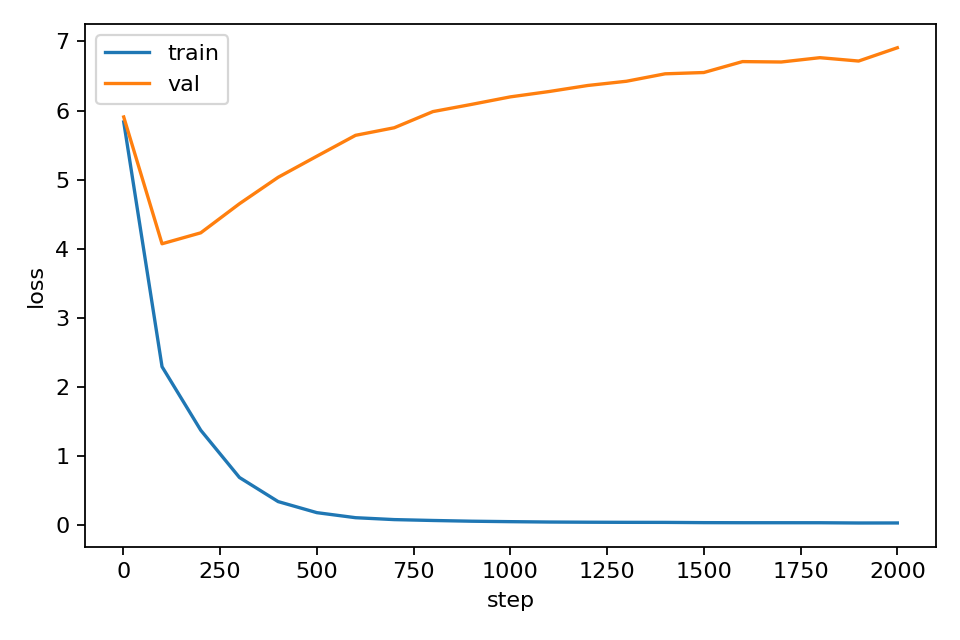
\includegraphics[width=\columnwidth]{work5_scratch_curves.png}
\caption{《孙子算经》从头训练损失曲线}
\end{figure}

\begin{table}[H]
\centering
\scriptsize
\caption{SFT 与 DPO 生成对比}
\resizebox{\columnwidth}{!}{
\begin{tabular}{llll}
\toprule
题型 & 标准答案 & SFT 输出 & DPO 输出 \\
\midrule
物不知数 & 二十三 & 二十三 & 二十三 \\
鸡兔同笼 & 雉二十三，兔一十二 & 雉二十三，兔一十二 & 雉二十三，兔一十二 \\
三人共车 & 一十五車，三十九人 & 一十五車，三十九人 & 一十五車，三十九人 \\
佛书字数 & 一千八百二十七 & 一千八百二十七 & 一千八百二十七 \\
车轮匝数 & 九萬匝 & 九萬匝 & 九萬匝 \\
\bottomrule
\end{tabular}}
\end{table}

\subsection{结果分析}

SFT 与 DPO 生成对比显示，模型在若干代表性题目上能输出简短的古文答案。例如“物不知数”输出“二十三”，“鸡兔同笼”输出“雉二十三。兔一十二。”，“车轮匝数”输出“九萬匝。”这些样例说明，预训练大模型的中文和数学先验使其比从头训练基线更容易适配古文题答格式。

本报告最有价值的地方在于，它没有把生成正确样例直接解释为“模型会推理”。《孙子算经》题答对数量较少，训练集与测试题型之间存在重复，模型可能学习到的是题目模板和答案记忆。自动扰动得到的偏好数据也比人工偏好标注粗糙，只能约束明显错误的数字和单位。因而，SFT 和 DPO 的结论应当理解为：预训练模型能在小语料上快速学会领域表达方式，偏好后训练可以进一步约束输出形式；但要证明严格算术泛化，还需要独立构造新数字、新组合和新题型的测试集。

从结果曲线看，从头训练基线具有典型的小语料过拟合特征：训练损失快速下降，而验证损失持续上升。这与报告二中的 LSTM 现象相呼应，只是在 Transformer 上表现得更明显。SFT 阶段的低训练损失说明模型很快适配了数据格式，但低训练损失本身不能证明泛化。DPO 阶段的调参记录也很重要：在小偏好集上训练过久会导致重复生成，说明后训练不是简单“步数越多越好”，而需要在偏好强度和语言流畅性之间保持平衡。

这一章与前两章的关系也很清楚。报告一证明了预训练在视觉任务中的收益，报告三则把同一思想迁移到语言模型：通用预训练模型已经包含大量中文表达和数学知识，领域微调主要负责把这些能力引导到特定格式中。报告二证明小模型可以学习领域模式，报告三则进一步说明，预训练大模型在同样小的数据条件下更容易生成可用答案，但也更容易让人误把格式正确看成推理正确。

\section{本课程经验总结}

回顾这三份报告，我对神经网络实验的认识从“跑出一个模型”逐渐转向“设计一个可信的比较”。Food101 实验让我看到，模型选择本身并不是最关键的问题，公平的对照设置、统一的数据增强、统一指标和训练时间记录，才是结论可信的基础。微调优于从头训练这一结果并不意外，但通过四组实验、收敛轮次和训练耗时把它定量化，才使结论具有工程价值。

《九章算术》和《孙子算经》两份文本实验则让我更清楚地认识到，生成模型的评价比分类任务困难。分类任务有 Accuracy 和 F1，错误边界比较明确；生成任务往往会出现“看起来像对的”输出。如果不设计 PPL、关键词命中率、近邻分析、chosen/rejected 对比和人工代表题，报告就容易停留在展示样例。因此，后续做语言模型实验时，我会优先考虑评价集如何构造，而不是先追求更复杂的模型。

从课程整体看，最重要的经验有三点。第一，预训练不是捷径，而是一种强先验；它能显著降低数据和算力压力，但仍需要通过任务内验证判断是否真的有效。第二，小模型并非没有价值；LSTM 和 Skip-gram 虽然能力有限，却更容易解释训练动态、过拟合边界和表示结构。第三，大模型微调不能只看少数成功样例；SFT 与 DPO 的输出需要和数据规模、偏好质量、测试集独立性一起讨论。

三份报告也让我对“完成度”有了更实际的理解。一个课程实验的完成度不只取决于代码是否能运行，还取决于是否保留了足够的实验记录。Food101 报告中，训练时长、验证准确率和测试指标让比较能够复核；《九章算术》报告中，曲线、困惑度、关键词命中率和生成样例互相补充；《孙子算经》报告中，从头训练、SFT、DPO 三阶段共同展示了同一数据在不同训练目标下的作用。以后做实验时，我会更早地设计日志、表格和图表，而不是在报告阶段再临时补证据。

\begin{table}[H]
\centering
\scriptsize
\caption{三份报告带来的课程经验}
\resizebox{\columnwidth}{!}{
\begin{tabular}{lll}
\toprule
经验 & 对应报告 & 启发 \\
\midrule
控制变量比单次高分更重要 & Food101 & 结论要能归因 \\
生成样例必须配合指标 & 《九章算术》 & 避免只看主观效果 \\
预训练能力需要边界说明 & 《孙子算经》 & 区分格式学习和推理 \\
日志和图表是实验资产 & 三份报告 & 报告质量来自过程记录 \\
\bottomrule
\end{tabular}}
\end{table}

如果继续完善这些工作，我会优先做三类改进：在视觉分类中加入多随机种子和混淆矩阵，提升统计可靠性；在古文数学生成中构造数字替换测试集，区分记忆和推理；在大模型后训练中引入人工偏好标注或规则验证器，避免 DPO 只学习到表面格式。课程实验让我认识到，神经网络研究的难点并不只在模型结构，也在于如何把问题拆成可验证的假设，并用足够诚实的指标说明模型真正学到了什么。

总体而言，这三份报告从不同方向回答了同一个问题：在有限条件下，模型如何获得可用能力。视觉分类说明了预训练特征的迁移价值，古文语言模型说明了小模型对领域格式的学习能力，大模型微调说明了现代后训练流程的效率与风险。它们共同构成了我对人工神经网络课程的主要收获：模型不是孤立存在的，真正重要的是数据、目标、训练过程和评价方式之间是否形成闭环。

最后，从报告写作本身看，我也学到了一点：课程综合报告不应只是把原报告复制压缩，而要重新组织问题意识。原来的三份报告分别服务于三次作业，现在需要被整合成一篇完整文档，就必须在开头给出统一视角，在每章保留最有代表性的实验事实，并在结尾回到同一个课程经验。这样处理后，报告虽然压缩了代码细节和运行命令，但保留了实验设计、结果证据、局限分析和个人总结，更接近一篇完整论文的结构。

\end{document}
